%%%%%%%%%%%%%%%%%%%%%%%%%%%%%%%%%%%%%%%%%%%%%%%%%%%%%%%%%%%%%%%%
% %
% Due Date %
% Andrew Gibson %
% ECE 351 lab, Section 53 %
% Lab 2 %
% Due 7 Jan 2023 %
% User-Defined Functions %
%https://github.com/gibs0630/ECE351\_Code %
%https://github.com/gibs0630/ECE351\_Reports %
% %
%%%%%%%%%%%%%%%%%%%%%%%%%%%%%%%%%%%%%%%%%%%%%%%%%%%%%%%%%%%%%%%%

\documentclass[12pt,a4paper]{article}
\usepackage[utf8]{inputenc}
\usepackage[greek,english]{babel}
\usepackage{alphabeta} 
\usepackage[pdftex]{graphicx}
\usepackage[top=1in, bottom=1in, left=1in, right=1in]{geometry}
\linespread{1.06}
\setlength{\parskip}{8pt plus2pt minus2pt}
\widowpenalty 10000
\clubpenalty 10000
\newcommand{\eat}[1]{}
\newcommand{\HRule}{\rule{\linewidth}{0.5mm}}
\usepackage[official]{eurosym}
\usepackage{enumitem}
\setlist{nolistsep,noitemsep}
\usepackage[hidelinks]{hyperref}
\usepackage{cite}
\usepackage{lipsum}


\newcommand{\Q}{\bigskip\bfseries Q: }
\newcommand{\A}{\par\textbf{A:} \normalfont}

\hypersetup{colorlinks=true, linkcolor=black, urlcolor=blue}

\begin{document}
%===========================================================
\begin{titlepage}
\begin{center}
% Top 
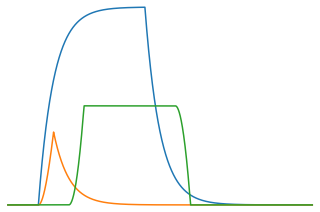
\includegraphics[width=0.55\textwidth]{titlepage_image.png}~\\[2cm]
% Title
\HRule \\[0.4cm]
{ \LARGE 
  \textbf{Project Report for ECE 351}\\[0.4cm]
  \emph{Lab 3: Discrete Convolution}\\[0.4cm]
}
\HRule \\[1.5cm]
% Author
{ \large
  Andrew Gibson \\[0.1cm]
  31 January 2023\\[0.1cm]
  \url{https://github.com/gibs0630/ECE351\_Code}\\[0.1cm]
  \url{https://github.com/gibs0630/ECE351\_Reports}\\[0.1cm]
  %#\texttt{user@cut.ac.cy}
}
\vfill
%\textsc{\Large Cyprus University of Technology}\\[0.4cm]\textsc{\large Department of Electrical Engineering,\\Computer Engineering \& Informatics}\\[0.4cm]
% Bottom
{\large }
 
\end{center}
\end{titlepage}
%\begin{abstract}
%\lipsum[1-2]
%\addtocontents{toc}{\protect\thispagestyle{empty}}
%\end{abstract}
\newpage
%===========================================================
\tableofcontents
\addtocontents{toc}{\protect\thispagestyle{empty}}
\newpage
\setcounter{page}{1}
%===========================================================
%===========================================================
\section{Introduction}\label{sec:intro}
Convolution is a function that will take two functions and output one function.
Computers store data in large arrays. With some specialized formatting, those arrays can be interpreted as coefficients to a function. however when given real world data, the data cannot be stored in such a way.  If it is known that an array is stored with a constant period between samples, then instead we can use Discrete Convolution. 

\section{Equations}\label{sec:lit-rev}
Formula's used
unit step function
\[
u(x) = \left\{
        \begin{array}{ll}
            0 & \quad t < 0 \\
            1 & \quad t \geq 0
        \end{array}
    \right.
\]
ramp function
\[
r(x) = \left\{
        \begin{array}{ll}
            0 & \quad t < 0 \\
            t & \quad t \geq 0
        \end{array}
    \right.
\]
discrete convolution with uniform time interval at 1
\[h(t) = \sum_{k=-\infty}^{\infty} {\left [ \sum_{n=0}^{k} {\left [ f_n*g_{k-n}* \Delta t\right ]} \right ]}\]

discrete convolution with uniform time intervals
\[h(t) = \sum_{k=-\infty}^{\infty} {\left [ \sum_{n=0}^{k} {\left [ f_n*g_{k-n}\right ]} \right ]}\]

functions from lab
\[f_1(t) = u(t-2)-u(t-9)\]
\[f_2(t) = e^{-t}*u(t)\]
\[f_3(t) = r(t-2)*(u(t-2)-u(t-3))+r(4-t)*(u(t-3)*u(t-4))\]


\section{Methodology}\label{sec:meth}
This lab had us develop a discrete convolution function using python.  Graphs were then created of convolved functions and then compared againsted a known good library, numpy. 

First an array of evenly spaced values for time, was created. Each of those discrete values of time were then plugged into a function of time to create various arrays.

The discrete convolution function was the created to convolve the functions using two for loops. The convolution was taken with the various arrays and plotted using the user defined convolve function. Same was done with the numpy's convolve.  The two were then subtracted to see any error between the two.

\section{Results}\label{sec:res}
\subsection*{Part 1}

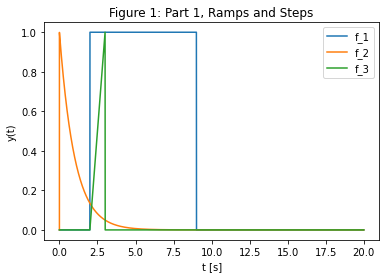
\includegraphics[width=0.55\textwidth]{Figure1.png}\\
The purpose producing Figure 1 was to show the functions as they are. Note that the y(t) are up to 1 here.

\subsection*{Part 2}
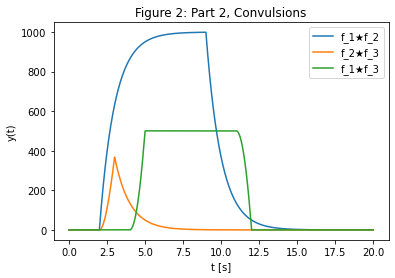
\includegraphics[width=0.55\textwidth]{Figure2.png}\\
Figure 2 shows the results with a user created created function.  Note that y(t) is up to 1000, that is because the time step interval was not 1 but was 0.001 when this data for this chart was calculated, yet the user defined function did not account for that.\\
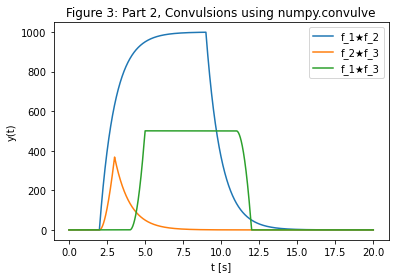
\includegraphics[width=0.55\textwidth]{Figure3.png}\\
Figure 3 shows the results with numpy's convolve function. however like figure 2, the built in  numpy's convolve function assumes that the time interval is 1.\\

\section{Error Analysis}\label{sec:res}
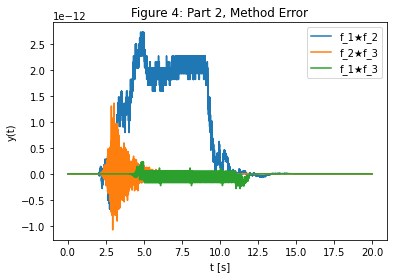
\includegraphics[width=0.55\textwidth]{Figure4.png}\\
Figure 4 is the subtraction of the user defined function and numpy's function when covnolving the same functions. Note that the deviation is less that 10E-12, which is a negligible difference and can be chalked up to boolean math rounding on the hardware.\\

As stated above, both of numpy's convolve functions and the user defined function both assume that the time interval is 1 wide, which cause values to skyrocket if the interval gets more densely packed as more data points are created.

\section{Questions}\label{sec:res}

\Q 1. Did you work alone or with classmates on this lab? If you collaborated to get to the solution, what did that process look like?
\A 1. I worked alone, but was given the formula for discrete convolution where the time interval is static. I implemented the formula with two for loops, however the return value was incorrect, as I made the error to sum over the wrong iterator ("y[i] += ", when I should have used "y[j] += ").

\Q 2. What was the most difficult part of this lab for you, and what did your problem-solving process look like?
\A 2.  the most difficult part of this lab was understanding the discrete convolution function.  Once I understood it i could create it via code. However, I also ran into issues where I was trying to use a sum function to use only one for loop, however that wouldn't have worked as I would have to edit/create new arrays each time it looped.

\Q 3. Did you approach writing the code with analytical or graphical
   convolution in mind? Why did you chose this approach?
\A 3. My approach was to treat each data point as a step function being added, which would have made things more confusing especially with a plethora ramps showing up that would have to be resolved.  That method went out the the window once I understood discrete convolution. My final approach would best be described as analytical.
\Q 4. Leave any feedback on the clarity of lab tasks, expectations, and deliverable.
\A 4.  This lab was strait forward, with the only thing missing was a that had to be solved was knowing what the discrete convolution was and how it is different from convolution.


\section{Conclusion}\label{sec:res}
When creating a function, it can be useful to generate a model and then run the numbers by hand to see if there is an error to the tools you are using.  By trying to increase the resolution, it had inadvertently changed the width because of the assumption of having each data point being separated by one unit wide.
Sometimes because some libraries do not account for certain scenarios in order to streamline themselves, it is often necessary to create your own functions that account for details that could be adjusted. (although typically it is better not to reinvent the wheel when it is good enough, but when there are multi-parameter adjustments it may be necessary.


%\lipsum[7-8]\cite{knuthwebsite}
%===========================================================
%===========================================================
\bibliographystyle{ieeetr}
\bibliography{refs}
\end{document} 
Annotations











